% !TEX TS-program = xelatex
%  encoding : utf8 
%  TKZdoc-aq.tex
% Copyright (C)  2021 Alain Matthes
% Copyright (C)  2019 Alain Matthes, Apostolos Syropoulos, and Anastasios Dimou
% Copyright (C)  2020 Alain Matthes
% This work may be distributed and/or modified under the
% conditions of the LaTeX Project Public License, either version 1.3
% of this license or (at your option) any later version.
% The latest version of this license is in
%   http://www.latex-project.org/lppl.txt
% and version 1.3 or later is part of all distributions of LaTeX
% version 2005/12/01 or later.
% This work has the LPPL maintenance status `maintained'.
% The Current Maintainer of this work is Alain Matthes
%
%
%%%%%%%%%%%%%%%%%%%%%%%%%%%%%%%%%%%%%%%%%%%%%%%%%%%%%%%%%%%%%%%%%
%                                                               %
%   doc   altermqcm.sty    encodage : utf8                      %
%                                                               %
%%%%%%%%%%%%%%%%%%%%%%%%%%%%%%%%%%%%%%%%%%%%%%%%%%%%%%%%%%%%%%%%%
%                                                               %
%           Créé par Alain Matthes le 30/05/2020                %
%  Copyright (c) 2020 __ AlterMundus __ All rights reserved.     %
%        version : 4.42                                         %
%%%%%%%%%%%%%%%%%%%%%%%%%%%%%%%%%%%%%%%%%%%%%%%%%%%%%%%%%%%%%%%%%

% Fichier  .tex de présentation du package alterqcm.sty
% d'après le code de DTK.
\documentclass[DIV=15,
               fontsize=10,
               headinclude=false,
               index=totoc,
               footinclude=false,
               twoside,
               headings=small
               ]{tkz-doc}
\usepackage{etoc}
\gdef\tkznameofpack{alterqcm}
\gdef\tkzversionofpack{4.42c}
\gdef\tkzdateofpack{2021/01/21}
\gdef\tkznameofdoc{doc-alterqcm}
\gdef\tkzversionofdoc{4.42c}   
\gdef\tkzdateofdoc{2021/01/21}
\gdef\tkzauthorofpack{Alain Matthes}
\gdef\tkzadressofauthor{}
\gdef\tkznamecollection{AlterMundus}
\gdef\tkzurlauthor{}
\gdef\tkzengine{xelatex}
\gdef\tkzurlauthorcom{http://altermundus.fr}
%\usepackage{xgreek}
\usepackage[dvipsnames,svgnames]{xcolor}
\usepackage{fancybox}
\usepackage{stmaryrd}
\usepackage{array,multirow,longtable}
\usepackage{tkz-tab,tkz-euclide,tkzexample}
\usepackage[english]{alterqcm}
\usepackage[colorlinks]{hyperref}
\hypersetup{   linkcolor=Gray,
                citecolor=Green,
                filecolor=Mulberry,
                urlcolor=NavyBlue,
                menucolor=Gray,
                runcolor=Mulberry,
                linkbordercolor=BrickRed,
                citebordercolor=Green,
                filebordercolor=Mulberry,
                urlbordercolor=NavyBlue,
                menubordercolor=Gray,
                runbordercolor=Mulberry,
                pdfsubject={qcm},
                pdfauthor={Alain Matthes},
                pdftitle={alterqcm},
                pdfkeywords={qcm, mathematics, table},
                pdfcreator={LaTeX}
                }

\usepackage{mathtools}
\usepackage{unicode-math,fourier-otf}
\setmainfont{Linux Libertine O}
\setmathfont[Scale=MatchUppercase]{Asana Math}
\setmonofont[Scale=MatchLowercase]{Consolas}
\usepackage{shortvrb,verbdef,fancyvrb,pifont}
\usepackage{multirow,multido,booktabs}
\usepackage[autolanguage]{numprint}
\usepackage{xeCJK}
\usepackage{textcomp}
\usepackage[all]{nowidow}
\widowpenalty10000
\clubpenalty10000
% %<––––––––––––––––––––––––––––––––––––––––––––––––––––––––––––––––––––––>
\renewcommand*{\Ienv}[1]{\index{%
Environnement_1@\texttt{Environnement}!\texttt{#1}}}
\renewcommand*{\NameSys}[1]{%
\index{Système d'exploitation !#1@\texttt{#1}}}
%\usepackage[parfill]{parskip}
%\renewcommand{\labelitemi}{\lefthand}
%<––––––––––––––––––––––––––––––––––––––––––––––––––––––––––––––––––––––>
\setlength\parindent{0pt}
\RequirePackage{makeidx}
%\def\tkzFileSavedPrefix{AQ}
\makeindex
\AtBeginDocument{\MakeShortVerb{\|}}
\def\lefthand{}
%\def\tkzHandBomb{}
\begin{document}
%<––––––––––––––––––––––––––––––––––––––––––––––––––––––––––––––––––––––>  
\author{\tkzauthorofpack}
\title{\tkznameofpack}
\date{\today}
\clearpage
\thispagestyle{empty}
\maketitle
\clearpage
\tkzSetUpColors[background=white,text=darkgray]
\let\rmfamily\ttfamily
\nameoffile{\tkznameofpack}

\defoffile{\tkzname{\tkznameofpack} (v 4.42 2020/08/17) Macros to support the creation of multiple-choice questionnaires in two-column tables. \tkzimp{Apostolos Syropoulos}, and \tkzimp{Anastasios Dimou} have adapted the package to use Greek. With the help of \tkzimp{Wolfgang Büchel} I added German, Russian and Italian. Finally it was \tkzimp{LianTze Lim} and \tkzimp{Chennan Zhang} who helped me with the Chinese translation. You can use another language with "unknown " option. With some languages, you need to compile with Xe\LaTeX. 
 \tkzname{alterqcm} is present on the \tkzname{CTAN} servers and is part of \tkzname{TeXLive} so \tkzname{tlmgr} or \tkzname{TeX Live Utility} will allow you to install it. 
  You will also   find  \tkzname{alterqcm} in  \tkzname{MikTeX} under \tkzname{Windows XP}.
}

\presentation

\vspace*{2cm}

\lefthand\ I  thank \tkzimp{Jean-Côme Charpentier}, \tkzimp{Manuel Pégourié-Gonnard}, \tkzimp{Franck Pastor}, \tkzimp{Ulrike Fischer} and \tkzimp{Josselin Noirel} for the different ideas and advices that allowed me to make this package. Thanks also to \tkzimp{Wolfgang Büchel} for his corrections and scripts.

\vfill
You can send your remarks, and reports on errors you have found.
 at the following address \href{mailto:al.ma@mac.com}{\textcolor{blue}{Alain} Matthes}


 This work may be distributed and/or modified under the
 conditions of the LaTeX Project Public License, either version 1.3
 of this license or (at your option) any later version.

This work has the LPPL maintenance status `maintained'.

The Current Maintainer of this work is Alain Matthes.


\clearpage\newpage
\setlength{\parskip}{1ex plus 0.5ex minus 0.2ex}

\tableofcontents
%<–––––––––––––––––––––––––––––––––––––––––––––––––––––––––––––––––––––––––––> 
%\section{Installation}

\subsection{Without \tkzNameDist{TeXlive} or \tkzNameDist{MikTeX}}
Create a folder and put your files, images and the \tkzname{alterqcm.sty} file in it. All you have to do is compile ...

\subsection{With \tkzNameDist{TeXlive} on \tkzNameSys{Linux} or \tkzNameSys{OS X}}

\tkzname{alterqcm} is present on the \tkzname{CTAN} servers and is part of \tkzname{TeXLive} so \tkzname{tlmgr} or \tkzname{TeX Live Utility} will allow you to install it.  If \tkzname{alterqcm} is not yet part of your distribution, this section shows you how to install it, it is also necessary if you want to install a beta or custom version of \tkzname{alterqcm}. 

The easiest way is to create a folder \tikz[remember picture,baseline=(n1.base)]\node [fill=blue!30,draw] (n1) {prof};\footnote{or another name} with as path: \colorbox{blue!20}{ texmf/tex/latex/prof}. Here are the paths to this folder on both my computers:

\medskip
\begin{itemize}\setlength{\itemsep}{5pt}

\item   with  \tkzNameSys{OS X} \colorbox{blue!30}{\textbf{/Users/ego/Library/texmf}}; 

\item   with  \tkzNameSys{OUnbuntu} \colorbox{blue!30}{\textbf{/home/ego/texmf}}.
\end{itemize}

I guess if you put your packages somewhere else, you know why! The concept is to place the package on a path that your distribution knows.


\medskip
\begin{enumerate}
\item Download the file \tikz[remember picture,baseline=(n2.base)]\node [fill=blue!20,draw] (n2) {alterqcm.sty}; from one of the servers of the \tkzname{CTAN}.

\item Place the file \tikz[remember picture,baseline=(n2.base)]\node [fill=blue!20,draw] (n2) {alterqcm.sty}; in the folder \tkzname{latex} or in a personal folder \tikz[baseline=(tk.base)]\node [fill=blue!30,draw] (tk) {prof};.
\begin{itemize}\setlength{\itemsep}{5pt}

\item  \colorbox{blue!30}{\textbf{\textasciitilde/Library/texmf/latex}}; 

\item   \colorbox{blue!30}{\textbf{\textasciitilde/Library/texmf/latex/prof}}.
\end{itemize}   

\end{enumerate} 


\subsection{With \tkzNameDist{MikTeX} under \tkzNameSys{Windows XP}}


I don't know much about this system, but a user of my packages \tkzimp{Wolfgang Buechel} was kind enough to send me the following~:

To add \tkzname{alterqcm.sty} to MiKTeX~:

\begin{itemize}\setlength{\itemsep}{10pt}
  \item add a folder \tkzname{prof} to the folder
       \textcolor{blue!60!black}{\texttt{[MiKTeX-dir]/tex/latex}}
  \item copy the file \tkzname{alterqcm.sty} to the folder \tkzname{prof},
  \item update MiKTeX, to do this in the DOS shell run the command   \textbf{\textcolor{red}{|mktexlsr -u|}} 
  
   or choose \textcolor{red!50}{|Start/Programs/Miktex/Settings/General|}
   
    then press the  \textbf{\textcolor{red}{|Refresh FNDB|}}.
\end{itemize}      

\endinput


\section{How to use: first example}

You need to load the \NamePack{alterqcm.sty} with  |\usepackage[english]{alterqcm}|, if you want to use the english language. With some languages like Greek or Chinese you need to compile with Xe\LaTeX\ otherwise you can compile with Lua\LaTeX\ or PDF\LaTeX\ .

Just use an environment \tkzname{alterqcm} and the macro \tkzcname{AQquestion}, here is an example :


 \noindent
\begin{minipage}[c][][t]{.40\linewidth}
\begin{tkzexample}[code only,small]
 \documentclass[12pt]{article}
 \usepackage[english]{alterqcm}
 % or french ...
 \usepackage{fullpage}
 \parindent0pt
 \begin{document}
 \begin{alterqcm}
  \AQquestion{Question}{%
  {Proposition 1},
  {Proposition 2},
  {Proposition 3}}
 \end{alterqcm}
 \end{document}\end{tkzexample}
\end{minipage}\hfill \noindent
\begin{minipage}[c][][b]{.50\linewidth}
\textbf{alterqcm.sty} creates a new environment \textbf{alterqcm} which allows for a two-column table. One column on the left for the questions, the other for the different proposals.  The propositions are given in a list :

\tkzname{\{\{Proposition 1\},\\\{Proposition 2\},\\\{Proposition 3\}\}}.

 The number of propositions is between \tkzname{2} and \tkzname{5}.
\end{minipage}

\medskip
The result is:

\bigskip
  \begin{alterqcm}
  \AQquestion{Question}
  {%
  {Proposition 1},
  {Proposition 2},
  {Proposition 3}%
  }
  \end{alterqcm}

\medskip
 The total width of the array is equal to \tkzcname{textwidth}. By default the question column has the width \tkzname{100mm} plus a few millimeters ... introduced by the table. The width of the answers is equal to \tkzcname{textwidth} minus the width of the first column. \Imacro{textwidth}

The important point is that the height of the lines in the proposals is calculated automatically so that, on the one hand, the text of the proposals is placed correctly without touching the lines and, on the other hand, the text of the corresponding question can be included in its box. Precise positioning is obtained with the option \tkzname{pq}.

\subsection{Packages loaded by \tkzname{alterqcm.sty}}
The list of loaded packages is as follows:

\begin{tkzexample}[code only]
  \RequirePackage{xkeyval}[2005/11/25]
  \RequirePackage{calc}
  \RequirePackage{ifthen,forloop}
  \RequirePackage{array}
  \RequirePackage{multirow}
  \RequirePackage{pifont}
\end{tkzexample}


\tkzHandBomb\ You will need to load \tkzname{longtable.sty} if you wish to use the \tkzname{long} option for one of your arrays.

\tkzHandBomb\ You also need the macro \tkzcname{square}, it is either defined in the package \tkzname{fourier} or in the package.
\endinput
\section{Tools: The environment \tkzname{alterqcm} and the macro \tkzcname{AQquestion}}
\subsection{Environment \tkzname{alterqcm}}


\bigskip
\begin{NewEnvBox}{alterqcm}

\noindent Here is the list of available \tkzname{options} classified by category.

\medskip
\begin{tabular}{@{}Il Il Il@{}}
  \toprule
  \thead
Options                &Default & Definition                                \\ \midrule
\tbody
\multicolumn{2}{c}{\emph{\texttt{Dimensions}}} \\ \cmidrule(r){1-2}
\TOenvline{lq}        {100mm}  {width of the question column            }
\TOenvline{pq}        {0pt}    {vertical shift of the question       } \cmidrule(r){1-2}
\multicolumn{2}{c}{\emph{\texttt{Numbers}}} \\ \cmidrule(r){1-2}
\TOenvline{bonus}     {{0,5}}  {points for a correct answer      }
\TOenvline{malus}     {{0,25}} {points for wrong answer   }
\TOenvline{numbreak}  {0}    {to take over a split board          }
\TOenvline{points}  {empty}{ points awarded to the qcm in the margin} \cmidrule(r){1-2}
\multicolumn{2}{c}{\emph{\texttt{Macros}}} \\ \cmidrule(r){1-2}
\TOenvline{symb}      {\$\BS square\$} {symbol in front of the proposal     }
\TOenvline{corsymb}{\$\BS blacksquare\$}{symbol in front of the proposal    }
\TOenvline{numstyle}  {\BS arabic} {style of question numbering  }
\TOenvline{propstyle} {\BS alph} {style of proposal numbering }
\TOenvline{size}  {\BS normalsize} {font size           }
\TOenvline{afterpreskip}{\BS medskip} {skip after the presentation  }
\cmidrule(r){1-2}
\multicolumn{2}{c}{\emph{\texttt{Booleans}}} \\ \cmidrule(r){1-2}
\TOenvline{long} {true}     {longtable instead of tabular   }
\TOenvline{sep} {true}  {proposal separator}
\TOenvline{pre} {false}  {MCQ presentation          }
\TOenvline{VF} {false}  {MCQ in the form True or False }
\TOenvline{numprop}   {false}  {proposal numbering    }
\TOenvline{num}       {true}   {style of question numbering  }
\TOenvline{nosquare}  {false}   {sremoving the square of proposals     }
\TOenvline{title}     {false} {title suppression                    }
\TOenvline{correction}{false} {allows you to create an answer sheet                }
\TOenvline{alea}      {false}  {randomly place proposals     } \cmidrule(r){1-2}
\multicolumn{2}{c}{\emph{\texttt{Texts}}} \\ \cmidrule(r){1-2}
\TOenvline{tone}     {Questions} {column title 1                           }
\TOenvline{ttwo}     {R\'eponses} {column title 2     }
\TOenvline{language}  {french}  {french, english, german, greek, russian, italian, chinese, unknown }
 \bottomrule
\end{tabular}

\medskip

To create a \textcolor{red}{\texttt{MCQ}} use a \textcolor{red}{\texttt{alterqcm}} environment as well as the \textcolor{red}{ \addbs{AQquestion}} macro defined in the next section.
\end{NewEnvBox}

\subsection{The macro \tkzcname{AQquestion}}
\Imacro{AQquestion}

\begin{NewMacroBox}{AQquestion}{\oarg{local options}{\var{quest}}\{{\var{$\mathrm{prop}_1$}},\ldots,{\var{$\mathrm{prop}_n$}}\}}
This macro uses two arguments, the first defines the question, the second is a list that defines the propositions.

\medskip
\begin{tabular}{@{}Il Il Il@{}}  \toprule \thead
arguments                 & default & definition    \\
\midrule
\tbody
\TAline{quest}  {}     {issue definition}
\TAline{$\mathrm{prop}_i$}  {}     {i\th\ proposition}       \bottomrule
\end{tabular}

\medskip
Here is the list of options related to this macro.

\medskip
\begin{tabular}{@{}Il Il Il@{}}  \toprule \thead
options                 & default & definition                    \\ \midrule
\tbody
\TOline{pq}  {0pt}     {adjustment of the position of the question}
\TOline{br}  {1  }     {ranked list of correct answers  }           \bottomrule
\end{tabular}

\medskip

\end{NewMacroBox}




 \subsection{Using the \tkzname{minipage} environment to change the width of the table}
\Ienv{minipage}

\tkzHandBomb\ \begin{minipage}[c][][t]{.4\linewidth}
\begin{tkzltxexample}[small]
\begin{center}
\begin{minipage}{9cm}
\begin{alterqcm}[lq=5cm]
    ...
  \end{alterqcm}
\end{minipage}
\end{center}
\end{tkzltxexample}
\end{minipage}

\begin{minipage}[c][][t]{.6\linewidth}
\begin{alterqcm}[lq=5cm]
\AQquestion{Among the following proposals, which of the following allows for 
 to affirm that the exponential function admits for asymptote the right 
  from the equation $y = 0$?}
{%
{$\displaystyle\lim_{x \to +\infty} \text{e}^x = + \infty$},%
{$\displaystyle\lim_{x \to -\infty} \text{e}^x = 0$},%
{$\displaystyle\lim_{x \to +\infty} \dfrac{\text{e}^x}{x} = + \infty$}%
}

\AQquestion[]{exp$(\ln x) = x$ for any $x$ belonging to }
{%
{$\mathbf{R}$},%
{$\big]0~;~+ \infty\big[$},%
{$\big[0~;~+\infty\big[$}%
}\end{alterqcm}
\end{minipage}
%

\subsection{Temporary modification of \tkzcname{textwidth}}
\Imacro{textwidth}
 It is possible to use tables and other structures in the question code or proposals. An example is shown below:
 \newlength{\oldtextwidth}
\tkzHandBomb\ \begin{tkzltxexample}[small]
  \newlength{\oldtextwidth}
\end{tkzltxexample}

\medskip
  \setlength{\oldtextwidth}{\textwidth}
  \setlength{\textwidth}{14cm}
\begin{alterqcm}[language=english,lq=88mm,symb=$\Box$]
 \AQquestion{the matrix 
 \( M=\begin{pmatrix}
        0 & 1 \\
        1 & 1 \\
\end{pmatrix} \)  has for square}%
{%
{\(\begin{pmatrix}
        0 & 1 \\
        1 & 4 \\
\end{pmatrix}\)},%
{\(\begin{pmatrix}
        1 & 2 \\
        2 & 5 \\
 \end{pmatrix}\)}
}
\end{alterqcm}
\setlength{\textwidth}{\oldtextwidth}

\medskip
\begin{tkzltxexample}[small]
  \setlength{\oldtextwidth}{\textwidth}
  \setlength{\textwidth}{14cm}
 \begin{alterqcm}[language=english,lq=88mm,symb=$\Box$]
  \AQquestion{la matrice %
  \( M=\begin{pmatrix}
         0 & 1 \\
         1 & 1 \\
 \end{pmatrix} \)  a pour carré}%
 {%
 {\(\begin{pmatrix}
         0 & 1 \\
         1 & 4 \\
 \end{pmatrix}\)},%
 {\(\begin{pmatrix}
         1 & 2 \\
         2 & 5 \\
  \end{pmatrix}\)}
 }
 \end{alterqcm}
 \setlength{\textwidth}{\oldtextwidth}
\end{tkzltxexample}

\endinput
\section{Global Environment Options  \tkzname{alterqcm}}

\subsection{\tkzname{lq} : changing the width of the first column }
\IoptEnv{alterqcm}{lq}

\begin{alterqcm}[long,lq=110mm]
\AQquestion{Of the following proposals, which one allows of
 to assert that the exponential function admits for asymptote 
  the equation line $y = 0$ ?}
{{$\displaystyle\lim_{x \to +\infty} \text{e}^x = + \infty$},
{$\displaystyle\lim_{x \to -\infty} \text{e}^x = 0$},
{$\displaystyle\lim_{x \to +\infty} \dfrac{\text{e}^x}{x} = + \infty$}}

\AQquestion{exp$(\ln x) = x$ for any $x$ belonging to }
{{$\mathbb{R}$},
{$\big]0~;~+ \infty\big[$},
{$\big[0~;~+\infty\big[$}
}
\end{alterqcm}

\medskip
Let's look at the code needed to get this table. We need to place
\tkzcname{usepackage}\{alterqcm\} in the preamble. Note that only the width of the question column is provided |lq=100mm| and that this is optional. The number of propositions is here \textbf{3} but it can vary from one question to another.

\begin{tkzexample}[code only,small]
 \begin{alterqcm}[long,lq=110mm]
  \AQquestion{Of the following proposals, which one allows  of
  to assert that the exponential function admits for asymptote
    the equation line $y = 0$ ?}
  {{$\displaystyle\lim_{x \to +\infty} \text{e}^x = + \infty$},
  {$\displaystyle\lim_{x \to -\infty} \text{e}^x = 0$},
  {$\displaystyle\lim_{x \to +\infty} \dfrac{\text{e}^x}{x} = + \infty$}}
  
  \AQquestion[]{exp$(\ln x) = x$ for any $x$ belonging to }
  {{$\mathbb{R}$},
  {$\big]0~;~+ \infty\big[$},
  {$\big[0~;~+\infty\big[$}
  }
  \end{alterqcm}\end{tkzexample}



\subsection{\tkzname{pq} : global use }
 \IoptEnv{alterqcm}{pq}  

This time, it is necessary to move several questions, I placed a pq=2mm globally, that is to say like this~:

\tkzcname{begin\{alterqcm\}[lq=85mm,pq=2mm]}. 

\textbf{All} questions are affected by this option but some questions were well placed and should remain so, so locally I give them back a |pq=0mm|.

\medskip
\begin{alterqcm}[lq=85mm,pq=2mm]
\AQquestion{A bivariate statistical series. The values of $x$ are 1, 2, 5, 7, 11, 13 and a least squares regression line equation of $y$ to $x$ is $y = 1.35x +22.8$. The coordinates of the mean point are :}
{{$(6,5;30,575)$},
{$(32,575 ; 6,5)$},
{$(6,5 ; 31,575)$}}

\AQquestion{For any real $x$, the number \[\dfrac{\text{e}^x - 1}{\text{e}^x + 2}\hskip12pt \text{equal to :} \] }
{{$-\dfrac{1}{2}$},
{$\dfrac{\text{e}^{-x} - 1}{\text{e}^{-x} + 2}$},
{$\dfrac{1 - \text{e}^{-x}}{1 + 2\text{e}^{-x}}$}
}
\AQquestion{With I $= \displaystyle\int_{\ln 2}^{\ln 3} \dfrac{1}{\text{e}^x - 1}\,\text{d}x$ and J $ = \displaystyle\int_{\ln 2}^{\ln 3} \dfrac{\text{e}^x}{\text{e}^x - 1}\,\text{d}x$ \\ then the number I $-$ J equals}
{{$\ln \dfrac{2}{3}$},
{$\ln \dfrac{3}{2}$},
{$\dfrac{3}{2}$}
}
\end{alterqcm}

\begin{tkzexample}[code only,small]
 \begin{alterqcm}[lq=85mm,pq=2mm]
 \AQquestion{For any real $x$, the number \[\dfrac{\text{e}^x - 1}
 {\text{e}^x + 2}\hskip12pt \text{equal to :} \] }
 {{$-\dfrac{1}{2}$},
 {$\dfrac{\text{e}^{-x} - 1}{\text{e}^{-x} + 2}$},
 {$\dfrac{1 - \text{e}^{-x}}{1 + 2\text{e}^{-x}}$}}
 \end{alterqcm}
\end{tkzexample}


\subsection{\tkzname{TF} : True or False}
\IoptEnv{alterqcm}{TF}
V or F in french vrai ou faux !
There are only two proposals and the candidate must choose between \textbf{True} or \textbf{False} ou bien si vous préférez \textbf{Correct} and \textbf{Wrong}. This time the syntax has been streamlined. It is no longer necessary to write the list of proposals and it is enough to position \tkzname{VF} by placing in the options \tkzname{$VF$}.

 
\begin{minipage}[t][][b]{.45\linewidth}
Let $f$ be a function defined and derivable on the interval $\big[-3~;~+\infty\big[$, increasing over the intervals $\big[-3~;~-1\big]$ et $\big[2~;~+\infty\big[$ and decreasing over the interval $\big[-1~;~2\big]$.

 We note $f'$ its derivative function over the interval $[-3~;~+\infty[$.

The $\Gamma$ curve representative of the $f$ function is plotted below in an orthogonal coordinate system $\big(O,~\vec{\imath},~\vec{\jmath}\big)$.

It passes through point A$(-3~;~0)$ and admits for asymptote the $\Delta$ line of equation $y =  2x -5$.
\end{minipage}
\hfill
\begin{minipage}[t][][b]{.45\linewidth}
\null
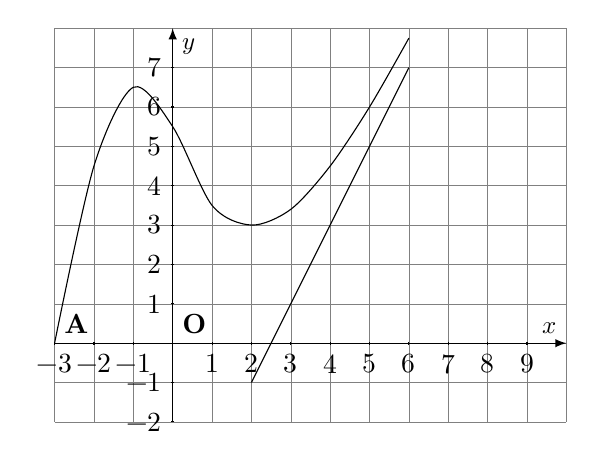
\begin{tikzpicture}[scale=0.5,>=latex]
 \draw[very thin,color=gray] (-3,-2) grid (10,8);
 \draw[->] (-3,0) -- (10,0) node[above left] {\small $x$};
 \foreach \x in {-3,-2,-1,1,2,...,9}
    \draw[shift={(\x,0)}] (0pt,1pt) -- (0pt,-1pt)node[below] { $\x$};
 \draw[->] (0,-2) -- (0,8) node[below right] {\small $y$};
 \foreach \y/\ytext in {-2,-1,1,2,...,7}
    \draw[shift={(0,\y)}] (1pt,0pt) -- (-1pt,0pt) node[left] { $\y$};
 \draw (2,-1) -- (6,7);
 \node[above right] at (-3,0) {\textbf{A}};
 \node[above right] at (0,0) {\textbf{O}};
 \node[below right] at (4,3) {$\mathbf{\Delta}$};
 \node[above right] at (4,5) {$\mathbf{\Gamma}$};
 \draw plot[smooth] coordinates{%
 (-3,0)(-2,4.5)(-1,6.5)(0,5.5)(1,3.5)(2,3)(3,3.4)(4,4.5)(5,6)(6,7.75)};
\end{tikzpicture}
\end{minipage}
                     

\begin{alterqcm}[VF,lq=125mm]
 \AQquestion{For all $x \in ]-3~;~2],~f'(x) \geqslant 0$.}
 \AQquestion{The $F$ function has a maximum in $2$}
 \AQquestion{$\displaystyle\int_{0}^2 f'(x)\,\text{d}x = - 2$}
\end{alterqcm}

\begin{tkzexample}[code only, small]
 \begin{minipage}[t][][b]{.45\linewidth}
  Let $f$ be a function defined and derivable on the interval $\big[-3~;~+\infty\big[$,
   increasing over the interval $\big[-3~;~-1\big]$ and $\big[2~;~+\infty\big[$
   and decreasing over the interval $\big[-1~;~2\big]$.
  
   We note $f'$ its derivative function over the interval $[-3~;~+\infty[$.
  
 The $\Gamma$ curve representative of the $f$ function is plotted below
   in an orthogonal system $\big(O,~\with{\imath},~\jmath}\big)$.
  
  It passes through the point A$(-3~;~0)$ and admits for asymptote the line
  $\Delta$ of equation $y = 2x -5$.
 \end{minipage}
 \begin{minipage}[t][][b]{.45\linewidth}
 \null
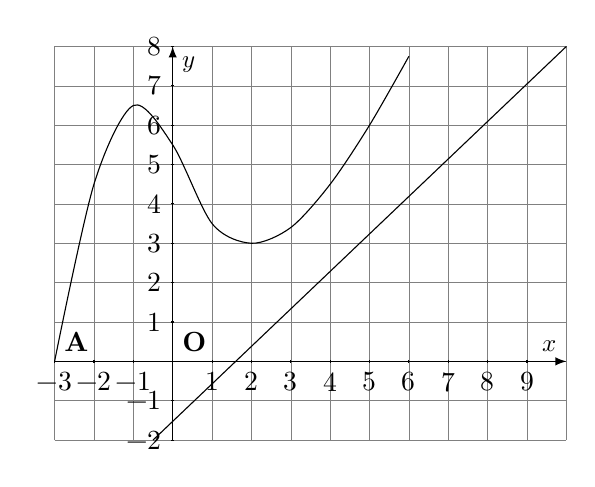
\begin{tikzpicture}[scale=0.5,>=latex]
  \draw[very thin,color=gray] (-3,-2) grid (10,8);
  \draw[->] (-3,0) -- (10,0) node[above left] {\small $x$};
  \foreach \x in {-3,-2,-1,1,2,...,9}
     \draw[shift={(\x,0)}] (0pt,1pt) -- (0pt,-1pt)node[below] { $\x$};
  \draw[->] (0,-2) -- (0,8) node[below right] {\small $y$};
  \foreach \y/\ytext in {-2,-1,1,2,...,8}
     \draw[shift={(0,\y)}] (1pt,0pt) -- (-1pt,0pt) node[left] { $\y$};
  \draw (-0.5,-2) -- (10,8);
  \node[above right] at (-3,0) {\textbf{A}};
  \node[above right] at (0,0) {\textbf{O}};
  \node[below right] at (4,3) {$\mathbf{\Delta}$};
  \node[above right] at (4,5) {$\mathbf{\Gamma}$};
  \draw plot[smooth] coordinates{%
  (-3,0)(-2,4.5)(-1,6.5)(0,5.5)(1,3.5)(2,3)(3,3.4)(4,4.5)(5,6)(6,7.75)};
 \end{tikzpicture}
 \end{minipage}
 \begin{alterqcm}[VF,lq=125mm]
   \AQquestion{For all $x \in ]-\infty~;~2],~f'(x) \geqslant 0$.}
   \AQquestion{The $F$ function has a maximum in $2$}
   \AQquestion{$\displaystyle\int_{0}^2 f'(x)\:\text{d}x = - 2$}
 \end{alterqcm}
\end{tkzexample}

\subsection{\tkzname{symb} : symbol change } 
\IoptEnv{alterqcm}{symb}

 If your fonts don't have the symbol |$\square$| or |$\blacksquare$| you can use the one provided by the package or create one yourself. \tkzcname{altersquare}, \tkzcname{dingsquare} and \tkzcname{dingchecksquare} are provided by alterqcm.
  Here is how these macros are defined.
  
\begin{tkzexample}[code only,small]
 \newcommand*{\altersquare}{\mbox{\vbox{\hrule\hbox to 6pt{\vrule height 5.2pt \hfil\vrule}\hrule}}}\end{tkzexample}

\medskip you either get \altersquare\ or... :

\begin{tkzexample}[code only,small]
 \newcommand*{\dingsquare}{\ding{114}} \end{tkzexample}

\medskip which results in \dingsquare\ and finally to replace |$\blacksquare$| 

\begin{tkzexample}[code only,small]
 \newcommand*{\dingchecksquare}{\mbox{\ding{114}%
 \hspace{-.7em}\raisebox{.2ex}[1ex]{\ding{51}}}} \end{tkzexample}

\medskip Let it be \dingchecksquare\ as a result. 


\begin{tkzexample}[code only,small] 

 \begin{alterqcm}[lq=90mm,symb=\altersquare]
 ... \end{alterqcm}\end{tkzexample}

\medskip
Full example :

\medskip
\begin{tkzexample}[vbox]
 \begin{alterqcm}[VF,lq=125mm,symb    = \dingsquare]
 \AQquestion{For all $x \in ]-3~;~2],~f'(x) \geqslant 0$.}
 \AQquestion{The $F$ function has a maximum in $2$}
 \AQquestion{$\displaystyle\int_{0}^2 f'(x)\:\text{d}x = - 2$}
 \end{alterqcm}\end{tkzexample}
  

\subsection{\tkzname{pre, bonus, malus} : automatic presentation }
\IoptEnv{alterqcm}{pre}\IoptEnv{alterqcm}{bonus}\IoptEnv{alterqcm}{malus}
As you can see below, a presentation is given of the exercise with the grading.

\bigskip
\begin{minipage}[c][][t]{.45\linewidth}
\begin{tkzexample}[code only,small]
  \begin{alterqcm}[lq=6cm,pre=true,bonus=1,malus={0,5}]
  \AQquestion{Question}
  {{Proposition 1},
   {Proposition 2}}
  \end{alterqcm}\end{tkzexample}
\end{minipage}\hfill
\begin{minipage}[c][][t]{.45\linewidth}
  \begin{alterqcm}[lq=3cm,pre=true,bonus=1,malus={0,5}]
  \AQquestion{Question}
  {{Proposition 1},
   {Proposition 2}}
  \end{alterqcm}
\end{minipage}

\vspace{1cm} 

\subsection{\tkzname{sep} : rule between proposals}
\IoptEnv{alterqcm}{sep}

\tkzname{sep=true} creates a rule between the proposals.

\begin{minipage}[c][][t]{.45\linewidth}
\begin{tkzexample}[code only,small]
  \begin{alterqcm}[lq=3cm,sep=true]
  \AQquestion{Question}
    etc..
\end{alterqcm}\end{tkzexample}
\end{minipage}\hfill
\begin{minipage}[c][][t]{.45\linewidth}
  \begin{alterqcm}[lq=3cm,sep=true]
  \AQquestion{Question}
  {{Proposition 1},
   {Proposition 2}}
  \end{alterqcm}
\end{minipage}

\subsection{\tkzname{num, numstyle} : deletion and style of numbering }
\IoptEnv{alterqcm}{num}\IoptEnv{alterqcm}{numstyle}
\subsubsection{\tkzname{num=false}}
\tkzname{num=false} makes the numbering of the questions disappear.

\begin{minipage}[c][][t]{.45\linewidth}
\begin{tkzexample}[code only, small]
  \begin{alterqcm}[lq=3cm,num=false]
    \AQquestion{Question}
     etc...
  \end{alterqcm}
\end{tkzexample}
\end{minipage}\hfill
\begin{minipage}[c][][t]{.45\linewidth}
  \begin{alterqcm}[lq=3cm,num=false]
  \AQquestion{Question}
  {%
  {Proposition 1},
  {Proposition 2}}
  \end{alterqcm}
\end{minipage}   

\subsubsection{\tkzname{numstyle}}   

\tkzname{numstyle}=\tkzcname{alph} changes the style of question numbering. The usual styles are valid here.

\begin{minipage}[c][][t]{.45\linewidth}
\begin{tkzexample}[code only, small]
 \begin{alterqcm}[lq=3cm,numstyle=\alph]
   \AQquestion{Question}
   etc...
 \end{alterqcm}
\end{tkzexample}  
\end{minipage}
\hfill
\begin{minipage}[c][][t]{.45\linewidth}
  \begin{alterqcm}[lq=3cm,numstyle=\alph]
  \AQquestion{Question}
  {%
  {Proposition 1},
  {Proposition 2}}
  \end{alterqcm}
\end{minipage}       
 
\subsection{\tkzname{title, tone, ttwo} : deletion and modification of the title line }
\IoptEnv{alterqcm}{title}\IoptEnv{alterqcm}{tone}\IoptEnv{alterqcm}{ttwo}

\tkzname{title=false} deletes the column headings.

\begin{minipage}[c][][t]{.45\linewidth}
\begin{tkzexample}[code only,vbox]
  \begin{alterqcm}[lq=3cm,title=false]
  \AQquestion{Question}
  etc...
  \end{alterqcm}\end{tkzexample}
\end{minipage}\hfill
\begin{minipage}[c][][t]{.45\linewidth}
  \begin{alterqcm}[lq=3cm,title=false]
  \AQquestion{Question}
  {%
  {Proposition 1},
  {Proposition 2}%
  }
  \end{alterqcm}
\end{minipage}
                      

\medskip
\tkzname{tone=titre n°1} and \tkzname{ttwo=titre n°2} change the table headers

\begin{minipage}[c][][t]{.45\linewidth}
\begin{tkzexample}[code only]
  \begin{alterqcm}[lq=3cm,tone=titre n°1,ttwo=titre n°2]
  \AQquestion{Question}
  etc...
  \end{alterqcm}\end{tkzexample}
\end{minipage}\hfill
\begin{minipage}[c][][t]{.45\linewidth}
  \begin{alterqcm}[lq = 3cm,tone = titre n°1,ttwo = titre n°2]
  \AQquestion{Question}
  {{Proposition 1},
   {Proposition 2}
  }
  \end{alterqcm}
\end{minipage}

\subsection{\tkzname{noquare} : square suppression }
\IoptEnv{alterqcm}{nosquare}

\tkzname{nosquare=true} fait disparaître le carré ou encore la numérotation des propositions.

\begin{minipage}[c][][t]{.45\linewidth}
\begin{tkzexample}[code only,small]
  \begin{alterqcm}[lq=3cm,nosquare=true]
  \AQquestion{Question}
  etc...
  \end{alterqcm}\end{tkzexample}
\end{minipage}\hfill
\begin{minipage}[c][][t]{.45\linewidth}
  \begin{alterqcm}[lq=3cm,nosquare=true]
  \AQquestion{Question}
  {%
  {Proposition 1},
  {Proposition 2}
  }
  \end{alterqcm}
\end{minipage}

\medskip
\tkzname{numprop=true} number the proposals and \tkzname{propstyle= ...} changes the numbering style.

Default, \tkzname{propstyle=\textbackslash alph}

\begin{minipage}[c][][t]{.45\linewidth}
\begin{tkzexample}[code only,small]
  \begin{alterqcm}[lq=3cm,numprop   = true,propstyle = \Roman]
  \AQquestion{Question}
  etc...
  \end{alterqcm}\end{tkzexample}
\end{minipage}\hfill
\begin{minipage}[c][][t]{.45\linewidth}
  \begin{alterqcm}%
  [lq=3cm,
   numprop   = true,
   propstyle = \Roman]
  \AQquestion{Question}
  {%
  {Proposition 1},
  {Proposition 2}%
  }
  \end{alterqcm}
\end{minipage}

\subsection{\tkzname{alea} : random positioning of proposals }
\IoptEnv{alterqcm}{alea}

It is preferable between two compilations to delete the auxiliary files.

\textcolor{red}{\lefthand} Be careful, in random mode, it is not possible to obtain an answer corresponding to the initial assignment.

\begin{tkzexample}[small]
 \begin{alterqcm}[lq=55mm,alea]
 \AQquestion[pq=1mm]{If the $f$ function is strictly increasing on  $\mathbf{R}$ then the equation $f(x) = $0 admits :}
 {{At least one solution},%
 {At most one solution},%
 {Exactly one solution}}
 \end{alterqcm}
\end{tkzexample}

\subsection{\tkzname{english}, \tkzname{german}, \tkzname{greek}, \tkzname{italian}, \tkzname{russian}, \tkzname{chinese}\ and \tkzname{unknown} : language change }
\IoptEnv{alterqcm}{english}\IoptEnv{alterqcm}{german}\IoptEnv{alterqcm}{french}

The order given above is that of creation.
Thanks to Apostolos Syropoulos and Anastasios Dimou for enabling the use of Greek language.

 \begin{tkzexample}[code only,small]
 \begin{alterqcm}[language=french,lq=55mm,alea] 
 \end{tkzexample}

 \begin{alterqcm}[language=french,lq=55mm,alea]
 \AQquestion[pq=1mm]{If the $f$ function is strictly increasing on $\mathbf{R}$
 then the equation equation $f(x) = $0 admits...}
 {{At least one solution},%
 {At most one solution},%
 {Exactly one solution}}
 \end{alterqcm}

 \begin{tkzexample}[code only,small]
 \begin{alterqcm}[language=german,lq=55mm,alea]  \end{tkzexample}

\begin{alterqcm}[language=german,lq=55mm,alea]
\AQquestion[pq=1mm]{Wenn die Funktion $f$ %
 auf $\mathbf{R}$ streng monoton wächst, dann
hat die Gleichung $f(x) = 0$:}
{{mindestens ein Lösung},%
{höchstens eine Lösung},%
{genau eine Lösung}}
\end{alterqcm}


\begin{alterqcm}[language=chinese,VF,lq=125mm,symb = \dingsquare,pre=true]
\def\aq@pre{对于以下提出的各个问题，仅有一个答案是正确的，请选择你认为正确的答案（不需要提供理由）。}
  \AQquestion{$x \in ]-3~;~2]$的情形下，$f'(x) \geq 0$。}
  \AQquestion{$F$ 函数的最大值为$2$。}
  \AQquestion{$\displaystyle\int_{0}^2 f’(x)\:\text{d}x = - 2$}
  \end{alterqcm}

  \begin{alterqcm}[language=chinese,pre=true]
  \AQquestion{问题}{%
  {选择1},
  {选择2},
  {选择3}}
  \end{alterqcm}


There's a section devoted solely to the "greek" option.


How to use \tkzname{unknown} : You need to call the package with the option "unknown" then yo need to redefine some macros. 

\begin{tkzexample}[code only,small]
\usepackage[unknown]{alterqcm}
% userdefined language: unknown=spanish
\def\aqlabelforquest{Preguntas}%
\def\aqlabelforrep{Respuestas}%
\def\aqtextfortrue{\textbf{V}}
\def\aqtextforfalse{\textbf{F}}
\def\txttv{V}% V(erdadero)
\def\txttf{F}% F(also)
\def\aqfoottext{Continúa en la página siguiente\dots}
\def\aqpretxt{\vspace*{6pt}Para cada una de las preguntas siguientes, sólo una de las respuestas propuestas es verdadera. Debe elegir la respuesta correcta sin justificación.}%
\def\aqpretxtVF{Para cada una de las afirmaciones de abajo, marque la casilla \textbf{V} (la afirmación es verdadera) o la casilla \textbf{F} (la afirmación es falsa).}%

\begin{alterqcm}[language=unknown]
 \AQquestion{Question}{%
 {Proposition 1},
 {Proposition 2},
 {Proposition 3}}
\end{alterqcm}

 \end{tkzexample}
\begingroup
\def\aqlabelforquest{Preguntas}%
\def\aqlabelforrep{Respuestas}%
\def\aqtextfortrue{\textbf{V}}
\def\aqtextforfalse{\textbf{F}}
\def\txttv{V}% V(erdadero)
\def\txttf{F}% F(also)
\def\aqfoottext{Continúa en la página siguiente\dots}
\def\aqpretxt{\vspace*{6pt}Para cada una de las preguntas siguientes, sólo una de las respuestas propuestas es verdadera. Debe elegir la respuesta correcta sin justificación.}%
\def\aqpretxtVF{Para cada una de las afirmaciones de abajo, marque la casilla \textbf{V} (la afirmación es verdadera) o la casilla \textbf{F} (la afirmación es falsa).}%
 
 \begin{alterqcm}[language=unknown]
  \AQquestion{Question}{%
  {Proposition 1},
  {Proposition 2},
  {Proposition 3}}
 \end{alterqcm}
  \endgroup
 
 
\newpage
\subsection{\tkzname{long} : use of longtable}
\IoptEnv{alterqcm}{long}\Ienv{longtable}

A table can arrive at the end of the page and be cut or simply be very long.
This option allows you to use instead of a \tkzname{tabular} an environnement \tkzname{longtable}.


Here is an example from Pascal Bertolino.

\begin{alterqcm}[lq=80mm,long]

%--------------------------------------------------------------
\AQquestion{What was the precursor language of the C language?}
{{Fortran},
 {language B},
 {Basic}}

%--------------------------------------------------------------
\verbdef\argprop|int a = 3 ^ 4 ;|
\AQquestion{\argprop}
{{raises 3 to the power of 4},
 {makes an exclusive OR between 3 and 4},
 {is not a C}}

%--------------------------------------------------------------
\AQquestion{What is the correct syntax to shift the integer 8 bits to the left? \texttt{a} ?}
{{\texttt{b = lshift(a, 8) ;}},
 {\texttt{b = 8 << a ;}},
 {\texttt{b = a << 8 ;}}}

%--------------------------------------------------------------
\verbdef\argprop|{ printf ("hello") ; return 0 ; \}|
\AQquestion{The complete program :  \\
            \texttt{int main() \\
            ~~\argprop}}
{{display \texttt{hello}},
 {gives an error to the compilation},
 {gives an error in execution}}

%--------------------------------------------------------------
\verbdef\arg|float tab[10]|
\verbdef\propa|*tab|\global\let\propa\propa
\verbdef\propb|&tab|\global\let\propb\propb
\verbdef\propc|tab|\global\let\propc\propc
\AQquestion{Let's say the statement \arg ; \\The first real in the table is \ldots}
{{\propa},
 {\propb},
 {\propc}}

%--------------------------------------------------------------
\AQquestion{The line \texttt{printf("\%c", argv[2][0]) ;} of \texttt{main} of  \texttt{monProg} run like this :
\texttt{monProg parametre }}
{{displays \texttt{p}},
 {displays nothing},
 {can cause a crash}}
%--------------------------------------------------------------
\AQquestion{What is the memory size of a \texttt{long int} ?}
{{4 octets},
 {8 octets},
 {it depends \ldots}}
%--------------------------------------------------------------
\AQquestion{Following the declaration \texttt{int * i} ;}
{{\texttt{*i} is an address},
 {\texttt{*i} is an integer},
 {\texttt{*i} is a pointer}}
%--------------------------------------------------------------
\AQquestion{One of the following choices is not a standard library of the C}
{{\texttt{stdlib}},
 {\texttt{stdin}},
 {\texttt{math}}}
 %--------------------------------------------------------------
\end{alterqcm}

The beginning of the code is simply

\begin{tkzltxexample}[small]
  \begin{alterqcm}[lq=80mm,long]
  \AQquestion{What was the precursor language of the C language?}
  {{Fortran},
   {language B},
   {Basic}}
  \end{alterqcm}
\end{tkzltxexample}

\medskip
It is possible to modify the text that is placed at the end of the table. Just modify the command \tkzcname{aqfoottext}.

\begin{tkzltxexample}[small]
 \def\aqfoottext{continued on next page\ldots}
\end{tkzltxexample}

\subsection{\tkzname{numbreak} : split a mcq }
This option allows either to continue the numbering of the previous table.
This option was necessary before the use of the \tkzname{long} option.
 for tables split by a page break. It can now be used
  for a series of tables grouped together to obtain a single MCQ.

\begin{alterqcm}[lq=80mm,title=false,num=false,long]
  \AQquestion{What was the precursor language of the C language?}
  {{Fortran},
   {language B},
   {Basic}}

\verbdef\argprop|int a = 3 ^ 4 ;|
\AQquestion{\argprop}
  {{raises 3 to the power of 4},
   {makes an exclusive OR between 3 and 4},
   {is not a C-instruction}}
\end{alterqcm}

\begin{alterqcm}[lq=80mm,title=false,num=false,numbreak=2,long]
\AQquestion{After the declaration \texttt{int * i} ;}
{{\texttt{*i} is an address},
 {\texttt{*i} is an integer},
 {\texttt{*i} is a pointer}}

\AQquestion{One of the following choices is not a standard C library}
{{\texttt{stdlib}},
 {\texttt{stdin}},
 {\texttt{math}}}
\end{alterqcm}

the code for the beginning is :

\begin{tkzltxexample}[small]
  \begin{alterqcm}[lq=80mm,title=false,num=false,long]
  \AQquestion{What was the precursor language of the C language?}
  {{Fortran},
   {language B},
   {Basic}}

  \verbdef\argprop|int a = 3 ^ 4 ;|
  \AQquestion{\argprop}
  {{raises 3 to the power of 4},
   {makes an exclusive OR between 3 and 4},
   {is not a C-instruction}}
  \end{alterqcm}
\end{tkzltxexample}

For the second part, we set \tkzname{numbreak} to $2$ because the first board had $2$ questions. In a future version, we will not have to count the questions anymore.

\begin{tkzltxexample}[small]
  \begin{alterqcm}[lq=80mm,title=false,num=false,numbreak=2,long]
  \AQquestion{Following the declaration \texttt{int * i} ;}
  {{\texttt{*i} is an address},
   {\texttt{*i} is an integer},
   {\texttt{*i} is a pointer}}

  \AQquestion{One of the following choices is not a standard C library}
  {{\texttt{stdlib}},
   {\texttt{stdin}},
   {\texttt{math}}}
  \end{alterqcm}
\end{tkzltxexample}

\subsection{\tkzname{correction} : Correction of a mcq}
 \IoptEnv{alterqcm}{correction}

 It is possible to create an answer key by using the \tkzname{correction} option and indicating the correct answer(s) using a local parameter \tkzname{br}.
 Here is an example:

 \begin{alterqcm}[VF,lq=125mm,correction,
                  symb    = \dingsquare,
                  corsymb = \dingchecksquare]
 \AQquestion[br=1]{For all $x \in ]-3~;~2],~f'(x) \geqslant 0$.}
 \AQquestion[br=2]{The $F$ function has a maximum in $2$}
 \AQquestion[br=2]{$\displaystyle\int_{0}^2 f'(x)\:\text{d}x = - 2$}
 \end{alterqcm}

 \begin{tkzltxexample}[]
  \begin{alterqcm}[VF,lq=125mm,correction,
                   symb    = \dingsquare,
                   corsymb = \dingchecksquare]
  \AQquestion[br=1]{For all $x \in ]-3~;~2],~f'(x) \geqslant 0$.}
  \AQquestion[br=2]{The $F$ function has a maximum in $2$}
  \AQquestion[br=2]{$\displaystyle\int_{0}^2 f'(x)\:\text{d}x = - 2$}
  \end{alterqcm}
\end{tkzltxexample}

\subsection{Modification du symbole \tkzname{corsymb}}
 \IoptEnv{alterqcm}{corsymb}

\tkzcname{dingchecksquare} is provided by alterqcm.
 Here is how this macro is defined.

\begin{tkzexample}[code only,small]
 \newcommand*{\dingchecksquare}{\mbox{\ding{114}%
 \hspace{-.7em}\raisebox{.2ex}[1ex]{\ding{51}}}} \end{tkzexample}

\medskip Let's consider checksquare as a result.

\begin{tkzexample}[code only,small]
 \begin{alterqcm}[lq=90mm,symb=\altersquare,corsymb=\dingchecksquare]
   ...
 \end{alterqcm}
\end{tkzexample}

\medskip
Full example :

\medskip
 \begin{alterqcm}[VF,lq=125mm,correction,
                  symb    = \dingsquare,
                  corsymb = \dingchecksquare]
 \AQquestion[br=1]{For all $x \in ]-3~;~2],~f'(x) \geqslant 0$.}
 \AQquestion[br=2]{The $F$ function has a maximum in $2$}
 \AQquestion[br=2]{$\displaystyle\int_{0}^2 f'(x)\:\text{d}x = - 2$}
 \end{alterqcm}


\begin{tkzexample}[code only]
 \begin{alterqcm}[VF,lq=125mm,correction,
                  symb    = \dingsquare,
                  corsymb = \dingchecksquare]
 \AQquestion[br=1]{For any $x \in ]-3~;~2],~f'(x) \geqslant 0$.}
 \AQquestion[br=2]{The $F$ function has a maximum in $2$}
 \AQquestion[br=2]{$\displaystyle\int_{0}^2 f'(x)\:\text{d}x = - 2$}
 \end{alterqcm}
\end{tkzexample}

\subsection{\tkzname{br=\{\ldots\}} : corrected with several correct answers}
\Iopt{AQquestion}{br}

A list of correct answers is given
\begin{tkzexample}[vbox,small]
\begin{alterqcm}[correction]
\AQquestion[br={1,3}]{Question}
{%
{Proposition 1},
{Proposition 2},
{Proposition 3}%
}
\end{alterqcm}
\end{tkzexample}

\subsection{\tkzname{transparent} : creation of a transparent slide showing the answers.}
 \IoptEnv{alterqcm}{transparent}

 This macro makes it possible to create a document identical to the original but without the questions and with a circle indicating the good proposals.

 \begin{tkzexample}[vbox,small]
 \begin{alterqcm}[transparent,correction,corsymb=\dingchecksquare,lq=100mm]
 \AQquestion[br=2,pq=3mm]{Which of the following proposals is that
  which allows us to affirm that the exponential function admits for asymptote  the equation line  $y = 0$ ?}
 {{$\displaystyle\lim_{x \to +\infty} \dfrac{\text{e}^x}{x} = + \infty$},
 {$\displaystyle\lim_{x \to +\infty} \text{e}^x = + \infty$},
 {$\displaystyle\lim_{x \to -\infty} \text{e}^x = 0$}
 }

 \AQquestion[br={1,3}]{exp$(\ln x) = x$ for any $x$ belonging to }
 {{$\mathbf{R}$},
 {$\big]0~;~+ \infty\big[$},
 {$\big[0~;~+\infty\big[$}
 }

 \AQquestion[br={1,2}]{exp$(\ln x) = x$ for any $x$ belonging to }
 {{$\mathbf{R}$},
 {$\big]0~;~+ \infty\big[$},
 {$\big[0~;~+\infty\big[$}
 }\AQquestion[br=2,pq=3mm]{Which of the following proposals is that
  which allows us to affirm that the exponential function admits for asymptote
  the equation line $y = 0$ ?}
 {{$\displaystyle\lim_{x \to +\infty} \dfrac{\text{e}^x}{x} = + \infty$},
 {$\displaystyle\lim_{x \to +\infty} \text{e}^x = + \infty$},
 {$\displaystyle\lim_{x \to -\infty} \text{e}^x = 0$}
 }
 \end{alterqcm}
\end{tkzexample}
\endinput
\section{Local options of the macro  \tkzcname{AQquestion}}

\subsection{Local use of \tkzname{pq}}
\Iopt{AQquestion}{pq} 
 The following table is obtained with the options |lq=85mm| and |size=\wide|. The questions are misplaced. The local option \tkzname{pq} solves this problem, the text can be moved 1mm upwards with \tkzcname{AQquestion[pq=1mm]}. 
  and by |6mm| for the second.

\medskip 


 \begin{alterqcm}[lq=55mm,size=\large]

\AQquestion{If the function $f$ is strictly increasing on $\mathbf{R}$ then the equation $f(x) = 0$ admits :}
{{At least one solution},
[At most one solution],
{Exactly one solution}
}
\AQquestion{If the $f$ function is continuous and positive on $[a~ ;~ b]$ and $\mathcal{C}_{f}$ its representative curve in an orthogonal system. In units of area, the area $\mathcal{A}$ of the domain delimited by $\mathcal{C}_{f}$, the abscissa axis and the lines of equations $x = a$ 5 and $x = b$ is given by the formula : }
{%
{$\mathcal{A}= \displaystyle \int_{b}^a f(x)\ \text{d}x$},
{$\mathcal{A}= \displaystyle \int_{a}^b f(x)\ \text{d}x$},
{$\mathcal{A} = f(b) - f(a)$}}
\end{alterqcm}

\medskip 
\tkzname{Here is the corrected version}

\begin{alterqcm}[lq=55mm,size=\large]
\AQquestion[pq=1mm]{If the $f$ function is strictly increasing on
$\mathbf{R}$ then the equation $f(x) = 0$ admits...}
{{At least one solution},
{At most one solution},
{Exactly one solution}
}
\AQquestion[pq=6mm]{If the $f$ function is continuous and positive on $[a~ ;~ b]$
 and $\mathcal{C}_{f}$ its representative curve in an orthogonal system.
  In area units, the $\mathcal{A}$ area of the domain delimited by $\mathcal{C}_{f}$, the abscissa axis and the lines of equations $x = a$ and $x = b$ is given  by the formula: }
{{$\mathcal{A}= \displaystyle \int_{b}^a f(x)\ \text{d}x$},
{$\mathcal{A}= \displaystyle \int_{a}^b f(x)\ \text{d}x$},
{$\mathcal{A} = f(b) - f(a)$}
}
\end{alterqcm}

\medskip
\begin{tkzexample}[code only, small]
 \begin{alterqcm}[lq=55mm,size=\large]
 \AQquestion[pq=1mm]{If the $f$ function is strictly increasing on  $\mathbf{R}$
 then the equation $f(x) =0 $ admits...
 {{{At least one solution},
 [At most one solution],
 {Exactly one solution}}
\end{tkzexample}

\medskip
\begin{tkzexample}[code only, small]
 \AQquestion[pq=6mm]{If the $f$ function is continuous and positive on $[a~ ;~ b]$ and $\mathcal{C}_{f}$ its representative curve in an orthogonal system.
   In units of area, the area $\mathcal{A}$ of the domain delimited by $\mathcal{C}_{f}$, the abscissa axis and the lines of equations $x = a$ and $x = b$ is given by the formula: }
 {{$\mathcal{A}= \displaystyle \int_{b}^a f(x)\ \text{d}x$},
 {$\mathcal{A}= \displaystyle \int_{a}^b f(x)\ \text{d}x$},
 {$\mathcal{A} = f(b) - f(a)$}}
 \end{alterqcm}
\end{tkzexample}

\subsection{Global and local use of \tkzname{pq}}\
 \Iopt{AQquestion}{pq} \IoptEnv{alterqcm}{pq}
This time, it is necessary to move several questions, I placed a |pq=2mm| globally, that is to say like this :\tkzcname{begin\{alterqcm\}[lq=85mm,pq=2mm]}. \textbf{All} questions are affected by this option but some questions were well placed and should remain so, so locally I give them back a |pq=0mm|.

\medskip
\begin{alterqcm}[lq=85mm,pq=2mm]
\AQquestion{A bivariate statistical series. The values of $x$ are 1, 2, 5, 7, 11, 13 and a least squares regression line equation of $y$ to $x$ is $y = 1.35x +22.8$. The coordinates of the mean point are :}
{{$(6,5;30,575)$},
{$(32,575 ; 6,5)$},
{$(6,5 ; 31,575)$}}

\AQquestion[pq=0mm]{$(u_{n})$ is an arithmetic sequence of reason $-5$.\\ Which of these statements is true? }
{{For all $n,~  u_{n+1} - u_{n} = 5$},
{$u_{10}= u_{2}+ 40$},
{$u_{3} = u_{7} + 20$}
}
\AQquestion[pq=0mm]{Equality $\ln (x^2 - 1) = \ln (x - 1) + \ln (x+1)$ is true}
{{For all $x$ in  $]- \infty~;~-1[ \cup]1~;~+ \infty[$},
{For all $x$ in $\mathbf{R} - \{-1~ ;~ 1\}$.},
{For all $x$ in $]1~ ;~+\infty[$}
}
\AQquestion{For all $x$, the number \[\dfrac{\text{e}^x - 1}{\text{e}^x + 2}\hskip12pt \text{equal to :} \] }
{{$-\dfrac{1}{2}$},
{$\dfrac{\text{e}^{-x} - 1}{\text{e}^{-x} + 2}$},
{$\dfrac{1 - \text{e}^{-x}}{1 + 2\text{e}^{-x}}$}
}
\AQquestion{Let I $= \displaystyle\int_{\ln 2}^{\ln 3} \dfrac{1}{\text{e}^x - 1}\,\text{d}x$ and J $ = \displaystyle\int_{\ln 2}^{\ln 3} \dfrac{\text{e}^x}{\text{e}^x - 1}\,\text{d}x$ \\ then the number  I $-$ J is equal to}
{{$\ln \dfrac{2}{3}$},
{$\ln \dfrac{3}{2}$},
{$\dfrac{3}{2}$}
}
\end{alterqcm}

\medskip
\begin{tkzexample}[code only,vbox,small]
 \begin{alterqcm}[lq=85mm,pq=2mm]
  \AQquestion[pq=0mm]{Equality $\ln (x^2 - 1) = \ln (x - 1) + \ln (x+1)$
   is true}
  {{For all $x$ in  $]- \infty~;~-1[ \cup]1~;~+ \infty[$},
  {For all $x$ in $\mathbf{R} - \{-1~ ;~ 1\}$.},
  {For all $x$ in $]1~ ;~+\infty[$}}
  \AQquestion{For any real $x$, the number \[\dfrac{\text{e}^x - 1}
  {\text{e}^x + 2}\hskip12pt \text{equal to :} \] }
  {{$-\dfrac{1}{2}$},
  {$\dfrac{\text{e}^{-x} - 1}{\text{e}^{-x} + 2}$},
  {$\dfrac{1 - \text{e}^{-x}}{1 + 2\text{e}^{-x}}$}}
  \end{alterqcm}
 \end{tkzexample}


\subsection{\tkzname{correction} and \tkzname{br} : rank of good answer}
\Iopt{AQquestion}{br}  \Iopt{AQquestion}{correction}
First of all, it is necessary to ask for an answer key. To do this, just include the option \tkzname{correction} which is a boolean, thus set to \tkzname{true}. Then in each question, it is necessary to give the list of correct answers. For example, with \tkzname{br=1} or \tkzname{br=\{1,3\}}.

Here is the previous year's correction:

\medskip
\begin{tkzexample}[vbox,small]
\begin{alterqcm}[VF,correction,lq=125mm]
 \AQquestion[br=1]{For all $x \in ]-3~;~2],~f'(x) \geqslant 0$.}
 \AQquestion[br=2]{The $F$ function has a maximum in $2$}
 \AQquestion[br=2]{$\displaystyle\int_{0}^2 f'(x)\:\text{d}x = - 2$}
\end{alterqcm}
\end{tkzexample}


\endinput
\section{Complementary macros}

\subsection{\tkzcname{AQmessage} : two-column message} 

It allows to insert in the table on the two columns, additional information for the candidate. 

In the following table, it is necessary to give indications and clarifications on the statement. This is done using the command \tkzcname{AQmessage}. I have used the package \tkzname{tkz-tab.sty} for this message as well as \emph{\texttt{AQmessage}} for some proposals, in order to make the proposal fit on several lines. This is necessary if one does not want to leave the table or if one does not want to restrict the space given to the questions.
This shows that many environments can be used in questions, messages and proposals at the same time.

\begin{NewMacroBox}{AQmessage}{{\var{texte}}}

\begin{tabular}{@{}Il Il Il@{}}  \toprule \thead
argument                 & default & definition     \\ \midrule
\tbody
\TAline{texte}  {}     {corps du message}      
\bottomrule
\end{tabular}

\medskip
\emph{This macro uses only one argument~: the text of the message. It can contain any kind of environment except, unfortunately, an array designed with \tkzname{tablor}. However, it is possible to import an array designed with \tkzname{tablor} with the macro \tkzcname{includegraphics}\footnotemark.}
\end{NewMacroBox}\Imacro{includegraphics}

\footnotetext{package macro \tkzname{graphicx}}

\begin{alterqcm}[lq=80mm,pre=false]
\AQmessage{\begin{minipage}{15cm}
\vspace*{6pt}
 Let $f$ be a function defined and derivable over the interval $]-5~;~+\infty[$ whose table of variations is given below :
\begin{center}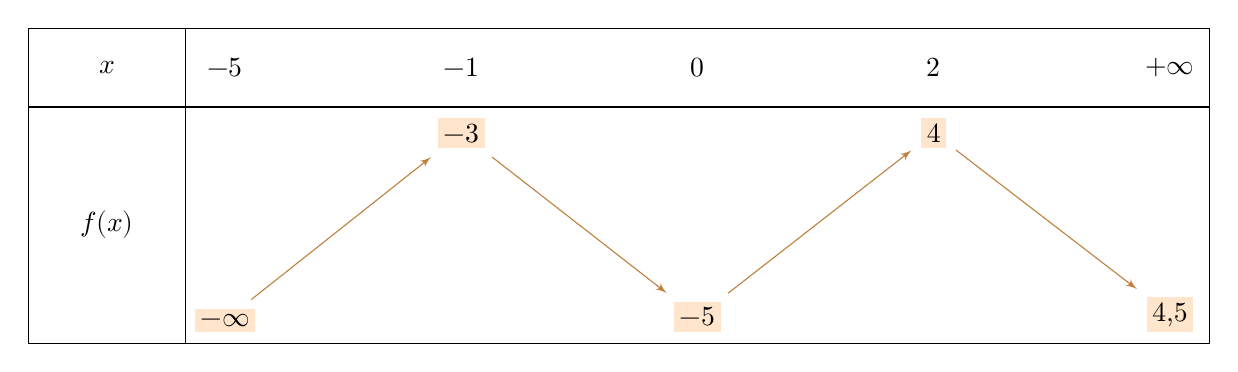
\begin{tikzpicture}
\def\tkzTabDefaultWritingColor{brown}
\def\tkzTabDefaultBackgroundColor{orange!20}  
\tkzTabInit{$x$/1,$f(x)$/3} {$-5$,$-1$,$0$,$2$,$+\infty$}
\tkzTabVar{-/$-\infty$ /,+/$-3$/,-/$-5$/,+/4/,-/{4,5}/}
\end{tikzpicture}\end{center}
 We designate by $\mathcal{C}$ the curve representative of $f$.
 \vspace*{6pt}    
\end{minipage} 
}
\AQquestion{In the interval $]-5~;~+\infty[$, the equation $f(x) = -2$ admits }
{{only one solution},
{two solutions},
{four solutions}}
\end{alterqcm}

\begin{tkzexample}[code only]
 \begin{alterqcm}[lq=95mm,pre=false]
  \AQmessage{ Let $f$ be a function defined and derivable on the interval%.
   $]-5~;~+\infty[$ whose table of variations is given below:
   \begin{center}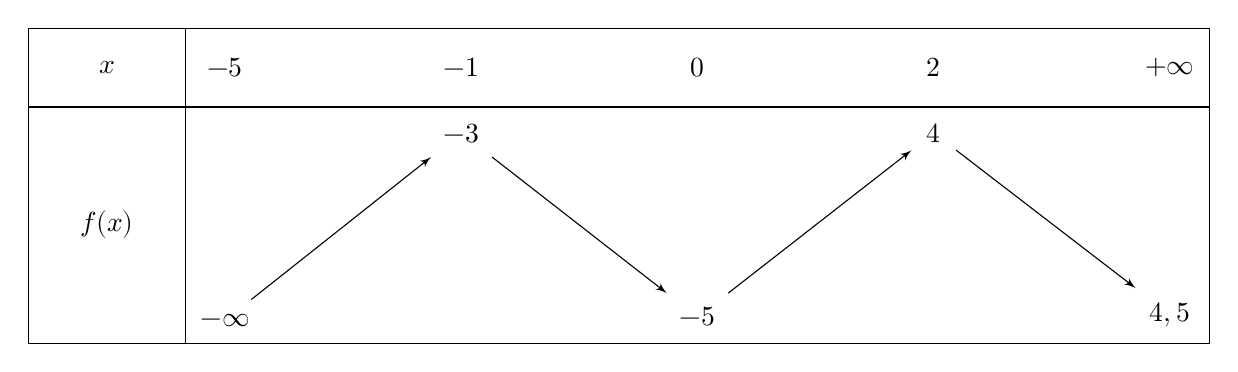
\begin{tikzpicture}
      \tkzTabInit{$x$/1,$f(x)$/3} {$-5$,$-1$,$0$,$2$,$+\infty$}
      \tkzTabVar{-/$-\infty$ ,+/$-3$,-/$-5$,+/$4$,-/${4,5}$}%
   \end{tikzpicture}\end{center}
  It is designated by $\mathcal{C}$  the curve representative of $f$.}
\AQquestion{Over the interval $]-5~;~+\infty[$,the equation $f(x) = -2$ admits}
  {{only one solution},
   {two solutions},
   {four solutions}}
 \end{alterqcm}\end{tkzexample}


\subsection{\tkzcname{AQms} : use of invisible line}

\begin{NewMacroBox}{AQms}{(height,depth)}
  \begin{tabular}{@{}Il Il Il@{}}  \toprule \thead
  argument                 & default & definition                    \\ \midrule
  \tbody
  \TAline{height}  {}     {line height}    
  \TAline{depth}  {}     {line depth}  
  \bottomrule
  \end{tabular}
  
\medskip
\emph{It's an invisible line useful if it is necessary to make more space around a proposal.}

\textcolor{red}{\emph{\texttt{ It should not be used!}}}
  
\end{NewMacroBox}
\footnotetext{ see the macro \tkzcname{strut}}

\begin{tkzexample}[code only,width=\textwidth-1pt]
 \def\AQms(#1,#2){\vrule height #1pt depth #2pt width 0pt} 
 \end{tkzexample}

\begin{tkzexample}[width=8cm]
  \begin{minipage}[]{7.5cm}
  \begin{alterqcm}%
  [lq=4cm]
  \AQquestion{Question}
   {%
  {Proposition 1},
  {Proposition 2\AQms(16,14)},
  {Proposition 3}}
  \end{alterqcm}
  \end{minipage}
\end{tkzexample}

\subsection{\tkzcname{InputQuestionList} : Multiple choice from a list of files}

\begin{NewMacroBox}{InputQuestionList}{\var{path}\var{prefix}\var{list of integers}}

\begin{tabular}{@{}Il Il Il@{}}  \toprule \thead
  argument                 & default & definition                    \\ \midrule
  \tbody
\TAline{path}  {}  {path that leads to the folder containing the files}       \TAline{prefix}  {} {file names  : <prefix><integer>.tex}          
\TAline{list of integers}{}{list of integers corresponding to the files} 
\bottomrule
 \end{tabular}
  
  \medskip  
\emph{This macro allows you to insert questions recorded in files into a table. A file can contain one or more questions with the corresponding propositions. \tkzname{path} is the path to the folder containing the files. \tkzname{prefix} is used to name the files, an integer uniquely determines the file.}

\end{NewMacroBox}

Let's say the file \tkzname{qcm-1.tex}

\begin{tkzltxexample}[]
\AQquestion{What was the precursor language of the C language?}
{{Fortran},
 {language B},
 {Basic}}
\end{tkzltxexample}

\medskip
Either the file \tkzname{qcm-2.tex}

\begin{tkzltxexample}[]
\verbdef\argprop|int a = 3 ^ 4 ;|
\AQquestion{\argprop}
{{raises 3 to the power of 4},
 {makes an exclusive OR between 3 and 4},
 {is not a C}}
\end{tkzltxexample}

\bigskip
Suppose we create a series of files in a folder \textbf{|iut|} with the following names \newline
 \tkzname{qcm-1.tex}, \tkzname{qcm-2.tex}, \ldots ,\tkzname{qcm-$n$.tex}. The prefix to name these files is \tkzname{qcm-}.

The path to this folder is for example 
|/examples/latex/iut/|.

The result is:

\newcommand*{\listpath}{/Users/ego/Desktop/waiting/alterqcm_new/examples/iut/}

\begin{alterqcm}[lq=80mm]
 \InputQuestionList{\listpath}{qcm-}{2,1}
\end{alterqcm}

\begin{tkzexample}[code only]
\newcommand*{\listpath}{/Users/ego/Desktop/waiting/alterqcm_new/examples/iut/}
\begin{alterqcm}[lq=80mm]
   \InputQuestionList{\listpath}{qcm-}{2,1}
\end{alterqcm}
\end{tkzexample}

\subsection{The command \tkzcname{AQannexe}} 


\begin{NewMacroBox}{AQannexe}{\oarg{local options}\var{start}\var{end}\var{col}}
\begin{tabular}{@{}Il Il Il@{}}  \toprule \thead
arguments        & default & definition                    \\ \midrule
\tbody
\TAline{start}    {}           {first row number}   
\TAline{end}      {}           {last row number}  
\TAline{col}      {}           {number of proposals}     
 \bottomrule
\end{tabular}

\medskip
\emph{This macro uses three arguments. These are three integers. \tkzname{start} is the row of the first row, \tkzname{end} is the final row and \tkzname{col} is the number of propositions. } 

\medskip
\begin{tabular}{@{}Il Il Il@{}}  \toprule \thead
Options     & default & definition        \\ \midrule
\tbody
\TOline{VF}         {false}          { true or false; displays T and F }    
\TOline{propstyle}  {\BS arabic}     { proposal numbering style }          \\
\bottomrule
\end{tabular}

\medskip
\emph{\tkzname{VF} allows to display V and F to identify the proposals but it is necessary that \tkzname{col} is equal to two}

\medskip

\end{NewMacroBox}

\begin{tkzltxexample}[]
  \documentclass{article} 
  \usepackage[utf8]{inputenc}
  \usepackage[T1]{fontenc}
  \usepackage{lmodern}
  \usepackage{alterqcm,fullpage}
  \thispagestyle{empty}

  \begin{document}
  NAME:

  FIRST NAME:

  \vspace{1cm}{ \Large
  \AQannexe{1}{10}{2}\hspace{2cm}
  \AQannexe[propstyle=\alph]{11}{20}{3}}
  \end{document}
\end{tkzltxexample}

\AQannexe{1}{10}{2}\hspace{2cm}
\AQannexe[propstyle=\alph]{11}{20}{3}
\endinput
\section{Additional examples} 
\subsection{The symbolists: use of the macro \tkzcname{includegraphics}}  
\Imacro{includegraphics}

\begin{alterqcm}[lq=8cm,numprop=true,sep]
\AQquestion[pq=2 cm]{Among the three paintings opposite, which is the one painted by \textbf{Gustave Moreau}\vfill}%
{{%
\hfil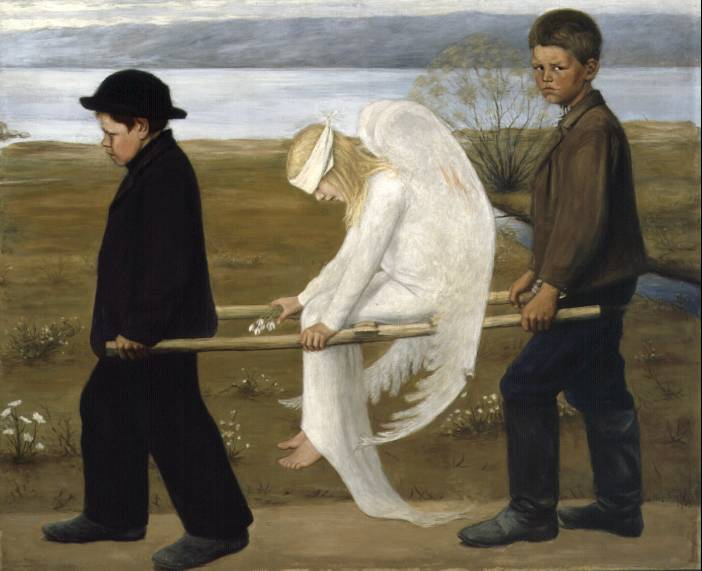
\includegraphics[scale=.20]{The_Wounded_Angel_-_Hugo_Simberg.jpg}\hfil
},{%
\hfil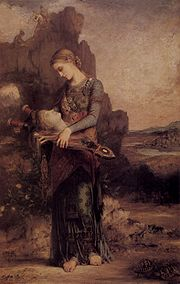
\includegraphics[scale=.4]{180px-Gustave_Moreau_007.jpg}\hfil
},{%
\hfil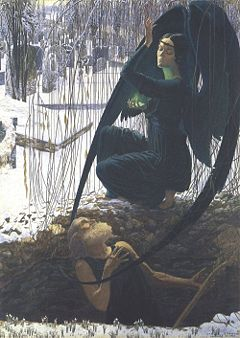
\includegraphics[scale=.4]{240px-Mort_du_fossoyeur.jpg}\hfil}}%
 \AQquestion[pq=1 cm]{The following picture was painted by which of these three painters?\\
\hfil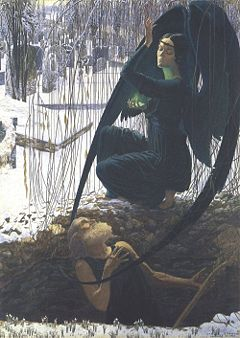
\includegraphics[height=3in]{240px-Mort_du_fossoyeur.jpg}\hfil}%
{{Gustav Klimt},{Carlos Schwabe},{Odilon Redon}}
\end{alterqcm} 

\begin{tkzltxexample}[small]
 \begin{alterqcm}[lq=8cm,numprop=true,sep]
 \AQquestion[pq=2 cm]{Of the three paintings, which is the one painted by \textbf{Gustave Moreau}\vfill}%
 {{%
 \hfil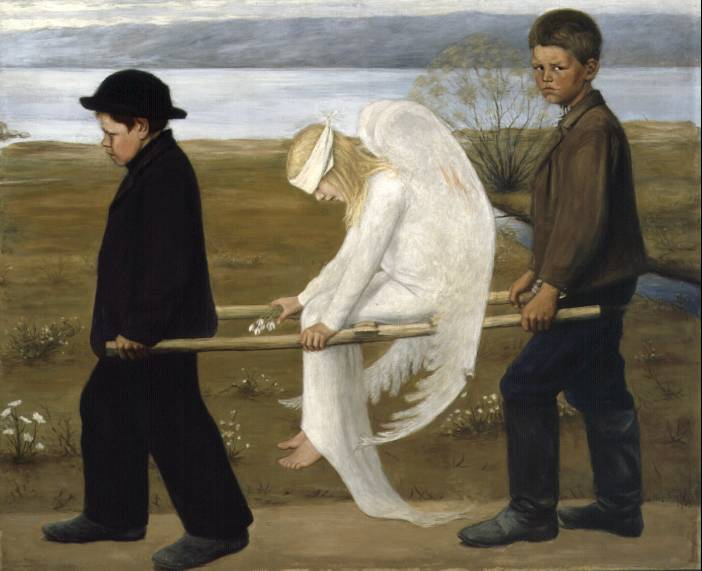
\includegraphics[scale=.25]{The_Wounded_Angel_-_Hugo_Simberg.jpg}\hfil
 },{%
 \hfil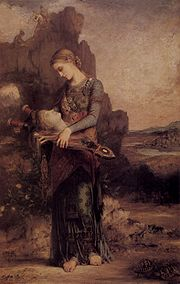
\includegraphics[scale=.5]{180px-Gustave_Moreau_007.jpg}\hfil
 },{%
 \hfil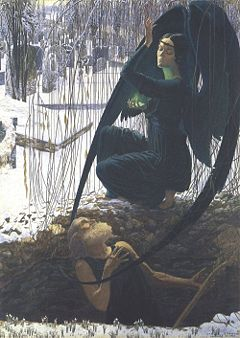
\includegraphics[scale=.4]{240px-Mort_du_fossoyeur.jpg}\hfil}}
  \AQquestion[pq=1 cm]{The following painting, was painted by which of these three painters?\\
 \hfil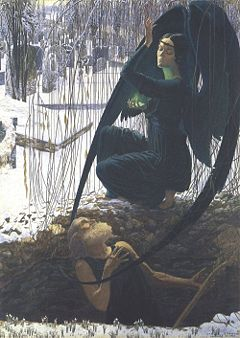
\includegraphics[height=3in]{240px-Mort_du_fossoyeur.jpg}\hfil}%
 {{Gustav Klimt},{Carlos Schwabe},{Odilon Redon}}
 \end{alterqcm} 
\end{tkzltxexample}

\subsection{Using a \tkzname{tikzpicture} environment in a question} 
\Ienv{tikzpicture}

\medskip

\begin{alterqcm}[lq=120mm,pre=true,pq=3mm]
 \AQmessage{\begin{minipage}{15cm}
\vspace*{6pt}   
The three trees given below represent probabilistic situations. %
  The numbers shown on the various arrows are probabilities, and,%.
    in the second level, conditional probabilities. Thus for the given tree %
      in question 1 : $0,35 = P(A)$ and $0,1 =  P_{\text{A}}(E)$.
\vspace*{6pt}    
\end{minipage}  
}
\AQquestion{The probability of event E is equal to : \\
\begin{tikzpicture}[yscale=1.2] 
[parent anchor=east,child anchor=west,grow=east]
\tikzstyle{every node}=[text=Maroon,fill=fondpaille,font=\small]
\tikzstyle{every child}=[level distance=25mm]
\tikzstyle{edge from parent}=[draw,->,thin] 
\tikzstyle{level 2}=[sibling distance=12mm]
\node {}
[grow=right]   
child {node {B}
      child { node {F}
        edge from parent node {$0,5$}}
      child { node {E}
        edge from parent node {$0,5$}
            }
         edge from parent node {$0,65$}
       }
child {node {A}
        child { node {F}
          edge from parentnode {$0,9$}}
        child { node {E}
          edge from parent node {$0,1$}}
      edge from parent node {$0,35$}
      };
\end{tikzpicture}}
{{$0,5$},%
{$0,1$},%
{$0,6$},%
{$0,36$}}
\end{alterqcm} 

\begin{tkzltxexample}[small]
 \begin{alterqcm}[lq=120mm,pre=true,pq=3mm]
  \AQmessage{The three trees given below represent probabilistic situations.
   The numbers shown on the different arrows are probabilities, and,
   in the second level, conditional probabilities. Thus for the given tree 
   in question 1: $0,35 = P(A)$ and $0,1 =  P_{\text{A}}(E)$.}
 \AQquestion{The probability of event E is equal to : \\
 \begin{tikzpicture} 
 ...
 \end{tikzpicture}}
 {{$0,5$},%
 {$0,1$},%
 {$0,6$},%
 {$0,36$}}
 \end{alterqcm} 
\end{tkzltxexample}

\begin{tkzexample}[vbox]
\begin{alterqcm}[lq=8cm,numprop=true,sep]
\AQquestion{Among the figures opposite, indicate the one that is a rhombus. :}
{{\hspace{1cm}  \begin{minipage}{5cm} 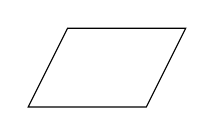
\begin{tikzpicture} 
  \draw (0,0)--(1.5,0)--(2,1)--(.5,1)--cycle; 
\end{tikzpicture} \end{minipage}},
{\hspace{1cm}  \begin{minipage}{5cm} 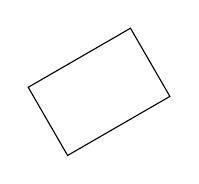
\begin{tikzpicture}
   \draw[rotate=30] (0,0) rectangle (1.5,1); \end{tikzpicture} \end{minipage}},
{\hspace{1cm}  \begin{minipage}{5cm} 
\begin{tikzpicture}
   \draw (0,0) rectangle (1,1); \end{tikzpicture} \end{minipage} }}
\end{alterqcm} 
\end{tkzexample}

\subsection{Use of a \tkzname{array} environment in the proposals} 
\Ienv{array}

It is possible to use tables and other structures in the question code or proposals. An example is shown below:

\medskip


\begin{tkzexample}[vbox]
\begin{alterqcm}[lq=88mm,symb=$\Box$]
\AQquestion{The couple $(1~;~-1)$ is a solution of }
{%
{$ \left\lbrace
\begin{array}{ll}
 0,75a + 0,5b &= 0,25 \\
 0,25a + 0,5b &=-0,25
\end{array}\right.$},
{$ \left\{
\begin{array}{ll}
 a &=  0,75a +0,5b \\
 b &=  0,25a +0,5b
\end{array}\right.$},
{$ \left\lbrace
\begin{array}{ll}
 0,75a - 0,5b &= 0,25 \\
 0,5a + 0,25b &=-0,25
\end{array}\right.$}
}
\end{alterqcm}\end{tkzexample}  


\subsection{Use of code \tkzname{verbatim} in questions and proposals} 
\Ienv{verbatim}

Here is an example from Pascal Bertolino. It is preferable to use as Pascal did the macro \tkzcname{texttt}, otherwise avoid the use of the mode 
|verbatim|. We will see on the next page how to proceed if this mode is really necessary.

\begin{alterqcm}[lq=80mm,title=false,long] 

%--------------------------------------------------------------
\AQquestion{What was the precursor language of the C language?}
{{Fortran},
 {Language B},
 {Basic}}

%--------------------------------------------------------------
\verbdef\argprop|int a = 3 ^ 4 ;|
\AQquestion{\argprop}
{{raises 3 to the power of 4},
 {makes an exclusive OR between 3 and 4},
 {is not a C}}

%--------------------------------------------------------------
\AQquestion{What is the correct syntax to shift the integer 8 bits to the left? \texttt{a} ?}
{{\texttt{b = lshift(a, 8) ;}},
 {\texttt{b = 8 << a ;}},
 {\texttt{b = a << 8 ;}}}
%--------------------------------------------------------------
\verbdef\argprop|{ printf ("hello") ; return 0 ; \}|
\AQquestion{The complete program:	\\
\texttt{int main() \\
~~\argprop}}
{{displays \texttt{hello}},
 {gives an error to the compilation},
 {gives an error in execution}}
%--------------------------------------------------------------
\verbdef\arg|float tab[10]|
\verbdef\propa|*tab|\global\let\propa\propa
\verbdef\propb|&tab|\global\let\propb\propb
\verbdef\propc|tab|\global\let\propc\propc
\AQquestion{Let's say the declaration \arg ; \\The first real in the table is \ldots}
{{\propa},
 {\propb},
 {\propc}}

%--------------------------------------------------------------
\AQquestion{The line \texttt{printf("\%c", argv[2][0]) ;}
 of \texttt{main} of  \texttt{monProg} run like this : 
\texttt{monProg parametre }}
{{displays \texttt{p}},
 {displays nothing},
 {can cause a crash}}
%--------------------------------------------------------------
\AQquestion{What is the memory size of a \texttt{long int} ?}
{{4 octets},
 {8 octets},
 {ça dépend \ldots}}
%--------------------------------------------------------------
\AQquestion{Following the declaration \texttt{int * i} ;}
{{\texttt{*i} is an address},
 {\texttt{*i} is an integer},
 {\texttt{*i} is a pointer}}
%--------------------------------------------------------------
\AQquestion{One of the following choices is not a standard C library}
{{\texttt{stdlib}},
 {\texttt{stdin}},
 {\texttt{math}}}

\end{alterqcm}

\medskip
Let's look at the source code

the simplest way is often to use the command \tkzcname{texttt}

\begin{tkzexample}[code only]
 \AQquestion{Following the declaration \texttt{int * i} ;}
 {{\texttt{*i} is an address},
 {\texttt{*i} is an integer},
 {\texttt{*i} is a pointer}}
\end{tkzexample}

\begin{tkzexample}[code only]
\AQquestion{The line \texttt{printf("\%c", argv[2][0]) ;}
 of \texttt{main} of  \texttt{monProg} run like this : 
\texttt{monProg parametre }}
{{displays \texttt{p}},
 {displays nothing},
 {can cause a crash}}
\end{tkzexample}

Alternatively, we can load the \tkzname{verbdef} package:
\tkzNamePack{verbdef}

\tkzcname{usepackage\{verbdef\}}

\begin{tkzexample}[code only]
 \verbdef\argprop|int a = 3 ^ 4 ;|
 \AQquestion{\argprop}
 {{raises 3 to the power of 4},
 {does an exclusive OR between 3 and 4},
  {is not a C-instruction}}
\end{tkzexample}

More than one variable may be required:

\begin{tkzexample}[code only]
 \verbdef\arg|float tab[10]|
 \verbdef\propa|*tab|\global\let\propa\propa
 \verbdef\propb|&tab|\global\let\propb\propb
 \verbdef\propc|tab|\global\let\propc\propc
 \AQquestion{Either the declaration  \arg ; \\
 The first real in the table is \ldots}
 {{\propa},
  {\propb},
  {\propc}}
\end{tkzexample}

\endinput
\section{Points assigned to an MCQ}

It is possible to assign points to an MCQ using the  rudimentary macro \tkzcname{AQpoints}.

  
\subsection{Example} 

 
\begin{tkzltxexample}[]
\AQpoints{10}
\begin{alterqcm}[symb = \dingsquare, lq=7cm]
  \AQquestion{If \numprint{3,24} is the truncation of $x$ to the hundredth..., then we're sure that :}
{%
  {\begin{minipage}[t]{\linewidth-1cm}
     $3,235\leqslant x <3,245$\\
   \end{minipage}} ,   
  {\begin{minipage}[t]{\linewidth-1cm} 
     $3,24\leqslant x <3,25$\\
    \end{minipage}} ,
  {\begin{minipage}[t]{\linewidth-1cm}
     $x$ is closer to \numprint{3,24} than \numprint{3,25}
   \end{minipage}}}
\end{alterqcm}
\end{tkzltxexample}

\medskip
\AQpoints{10}
  \begin{alterqcm}[symb = \dingsquare, lq=7cm]
  \AQquestion{Si \numprint{3,24} is the truncation of $x$ to the hundredth..., then we're sure that :}
  {{\begin{minipage}[t]{\linewidth-1cm}$3,235\leqslant x <3,245$\\
    \end{minipage}} ,
   {\begin{minipage}[t]{\linewidth-1cm} $3,24\leqslant x <3,25$\\
    \end{minipage}} ,
   {\begin{minipage}[t]{\linewidth-1cm}
       $x$ is closer to \numprint{3,24} than \numprint{3,25}
    \end{minipage}}}

\end{alterqcm}   
\endinput
\section{Known issues and FAQs}

\subsection{Incompatibility with \tkzname{colortbl.sty}}

 The problem is that \tkzname{colortbl.sty} is sometimes incompatible with the command \tkzname{multicolumn}. The text used in the \tkzname{multicolumn} command should contain only one paragraph. 
  Simply do not use the \tkzname{AQmessage} command. One solution is to interrupt the quiz to display what you want and then resume the table.
 
 \subsection{FAQ}
  \subsubsection{Translation of commands}
  Some commands can be translated or modified such as : \tkzcname{aq@pre} and \tkzcname{aq@preVF}, all you have to do is use \tkzcname{renewcommand} 
  
\begin{tkzltxexample}[]
\makeatletter
 \renewcommand{\aq@pre}{Pour chacune des questions ci-dessous, une seule des
  r\'eponses propos\'ees est exacte. Vous devez  cocher la r\'eponse exacte
   sans justification.
 Une bonne r\'eponse rapporte \textbf{\cmdAQ@global@bonus\ point}. Une
  mauvaise r\'eponse enl\`eve \textbf{\cmdAQ@global@malus\ point}.  L'absence
  de r\'eponse ne rapporte ni n'enl\`eve aucun point. Si le total des points
  est n\'egatif, la note globale attribu\'ee \`a l'exercice est \textbf{0}.}%
\makeatother 
\end{tkzltxexample}

  
\endinput
\section{Greek version [Apostolos Syropoulos \& Anastasios Dimou]}

\subsection{Εισαγωγή} 
Ο Alain Matthes μας έχει συνηθίσει σε ενδιαφέροντα πακέτα για το \LaTeX\ , που είναι μάλιστα πολύ σχετικά με τα δικά μας προγράμματα, το στυλ και το ύφος τους. Ένα τέτοιο παράδειγμα είναι και το \texttt{tkz-tab}, που παρουσιάστηκε πέρυσι στο \texttt{https://tassosdimou.gr/variation-table}.

Το πακέτο \textsf{alterqcm} είναι ακόμη ένα πακέτο του Alain Matthes για το \LaTeX\, που θα μας βοηθήσει στη κατασκευή καλαίσθητων διαγωνισμάτων με ερωτήσεις πολλαπλής επιλογής και σωστού-λάθους.

Το \textsf{alterqcm}  τροποποιήθηκε από τους Απόστολο Συρόπουλο και Τάσσο Δήμου έτσι, ώστε να προσαρμοστεί στα δεδομένα του ελληνικού εκπαιδευτικού συστήματος. 

 Το άρθρο αναπτύσσει με λεπτομέρειες και πολλά παραδείγματα τις δυνατότητες του \textsf{alterqcm}. Δίνει οδηγίες για τη χρήση του και στο τέλος  θα δοθούν μερικά παραδείγματα διαγωνισμάτων.

\subsection{Εγκατάσταση του πακέτου}	
Θα υποδείξουμε έναν απλό τρόπο εγκατάστασης του πακέτου. Δημιουργούμε ένα φάκελο, στον οποίο θα αποθηκευτούν όλα τα αρχεία, που θα επεξεργαστούμε, μελετώντας το \textsf{alterqcm}. Με άλλα λόγια, στον φάκελο αυτόν αποθηκεύουμε τα αρχεία \texttt{.tex}, τις εικόνες που θα χρησιμοποιηθούν και το αρχείο \texttt{alterqcm.sty}, που θα κατεβάσουμε από τη διεύθυνση \texttt{https://ctan.org/pkg/alterqcm?lang=en}. Το πακέτο θα φορτωθεί με την επιλογή \texttt{greek}, δηλαδή θα δώσουμε την εντολή:
\begin{verbatim}
\usepackage[greek]{alterqcm}
\end{verbatim}
Όλα τα αρχεία θα έχουν την κλασσική δομή των αρχείων \texttt{.tex}.

Στο πρώτο μέρος, το προοίμιο, θα τοποθετήσουμε τα: 
\begin{verbatim}
\documentclass[11pt,a4paper]{article}
\usepackage{xltxtra}
\usepackage{xgreek}
\usepackage{mathtools}
\usepackage{amsthm}
\usepackage{amssymb}
\usepackage{unicode-math}
\usepackage{xkeyval}
\usepackage{multirow,longtable}
\usepackage[greek]{alterqcm}
\usepackage{tkz-tab}
%%%%%%%%%%%%%%%%%%%%%%%%%%%%%%%%%%%%%%%%%%%%%%%%%%%%%%%%%
\parindent=0pt
\setmainfont[Mapping=tex-text,Ligatures=Common]{Minion Pro}
\setmathfont[Scale=MatchUppercase]{Asana Math}
\end{verbatim}	

Apostolos Syropoulos, and Anastasios Dimou

\begin{alterqcm}
  \AQquestion{Ερώτηση}{%
  {Επιλογή 1},
  {Επιλογή 2},
  {Επιλογή 3}
  }
 \end{alterqcm}
 
 \begin{alterqcm}[language=greek,VF,lq=60mm]
 \AQquestion[]{Ισχύει ότι $(α+β)^2=α^2+β^2$}
 \AQquestion[]{Αν $α\cdot β\geq 0$, τότε $\sqrt{α\cdot β}=\sqrt{α}\cdot\sqrt{β}$ } 
 \AQquestion[]{Είναι $|α|=α,\,\text{για κάθε}\ 
  x\in\mathbb{R}$}
 \end{alterqcm}
\clearpage\newpage
\begin{multicols}{2}
\small\printindex
\end{multicols}
\end{document}